%%%%%%%%%%%%%%%%%%%%%%%%%%%%%%%%%%%%%
%                                   %
% Compile with XeLaTeX and biber    %
%                                   %
% Questions or comments:            %
%                                   %
% joshua dot mcneill at uga dot edu %
%                                   %
%%%%%%%%%%%%%%%%%%%%%%%%%%%%%%%%%%%%%

\documentclass{beamer}
  % Read in standard preamble (cosmetic stuff)
  %%%%%%%%%%%%%%%%%%%%%%%%%%%%%%%%%%%%%%%%%%%%%%%%%%%%%%%%%%%%%%%%
% This is a standard preamble used in for all slide documents. %
% It basically contains cosmetic settings.                     %
%                                                              %
% Joshua McNeill                                               %
% joshua dot mcneill at uga dot edu                            %
%%%%%%%%%%%%%%%%%%%%%%%%%%%%%%%%%%%%%%%%%%%%%%%%%%%%%%%%%%%%%%%%

% Beamer settings
% \usetheme{Berkeley}
\usetheme{CambridgeUS}
% \usecolortheme{dove}
% \usecolortheme{rose}
\usecolortheme{seagull}
\usefonttheme{professionalfonts}
\usefonttheme{serif}
\setbeamertemplate{bibliography item}{}

% Packages and settings
\usepackage{fontspec}
  \setmainfont{Charis SIL}
\usepackage{hyperref}
  \hypersetup{colorlinks=true,
              allcolors=blue}
\usepackage{graphicx}
  \graphicspath{{../../figures/}}
\usepackage[normalem]{ulem}
\usepackage{enumerate}

% Document information
\author{M. McNeill}
\title[FREN2001]{Français 2001}
\institute{\url{joshua.mcneill@uga.edu}}
\date{}

%% Custom commands
% Lexical items
\newcommand{\lexi}[1]{\textit{#1}}
% Gloss
\newcommand{\gloss}[1]{`#1'}
\newcommand{\tinygloss}[1]{{\tiny`#1'}}
% Orthographic representations
\newcommand{\orth}[1]{$\langle$#1$\rangle$}
% Utterances (pragmatics)
\newcommand{\uttr}[1]{`#1'}
% Sentences (pragmatics)
\newcommand{\sent}[1]{\textit{#1}}
% Base dir for definitions
\newcommand{\defs}{../definitions}


  % Packages and settings

  % Document information
  \subtitle[Adjectifs prénominaux au pluriel]{Les adjectifs prénominaux au pluriel}

\begin{document}
  % Read in the standard intro slides (title page and table of contents)
  \begin{frame}
    \titlepage
    \tiny{Office: % Basically a variable for office hours location
Gilbert 121\\
          Office hours: % Basically a variable for office hours
 lundi, mercredi, vendredi 10:10--11:10
}
  \end{frame}

  \begin{frame}{}
    \begin{center}
      \Large Quiz
    \end{center}
  \end{frame}

  \begin{frame}{Décrivons l'université}
    \begin{columns}
      \column{0.5\textwidth}
        {\scriptsize
        \begin{enumerate}
          \item Il y a des (\only<1>{vieux}\only<2->{\underline{vieux}}, vieil, vieilles) amphithéatres.
          \item<3-> Voici des (bon, \only<3>{bons}\only<4->{\underline{bons}}, bonnes) laboratoires.
          \item<5-> Il a des (\only<5>{gros}\only<6->{\underline{gros}}, grosse, grosses) ordinateurs.
          \item<7-> Voici des (jeune, \only<7>{jeunes}\only<8->{\underline{jeunes}}) étudiants.
          \item<9-> Il y a des (bel, belles, \only<9>{beaux}\only<10->{\underline{beaux}}) terrains de sport.
          \item<11-> Ce sont des (\only<11>{grands}\only<12->{\underline{grands}}, grandes, grand) bureaux.
          \item<13-> Voici des (bel, beaux, \only<13>{belles}\only<14->{\underline{belles}}) affiches.
          \item<15-> Ce sont des (nouvel, \only<15>{nouvelles}\only<16->{\underline{nouvelles}}, nouveaux) navettes.
        \end{enumerate}
        }
      \column{0.5\textwidth}
        \begin{minipage}[c][0.6\textheight]{\linewidth}
          \begin{center}
            \only<-2>{
              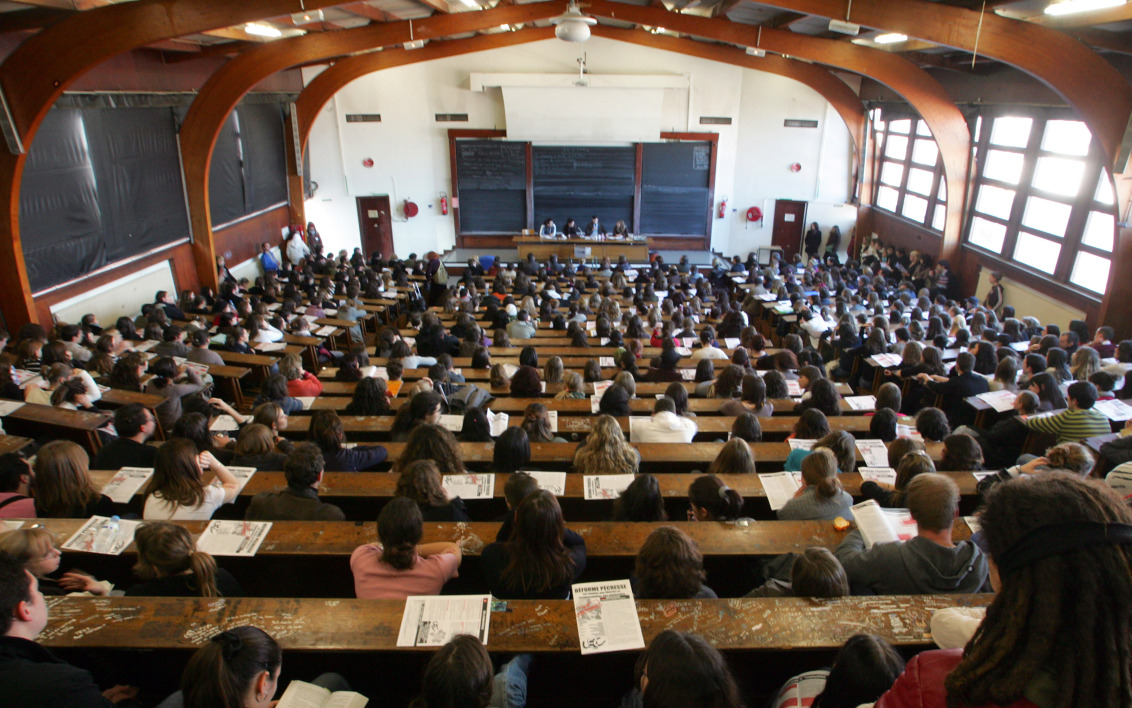
\includegraphics[scale=0.6]{amphitheatre.jpeg}
            }
            \only<3-4>{
              
\includegraphics[scale=0.38]{richards_lab.jpg}
            }
            \only<5-6>{
              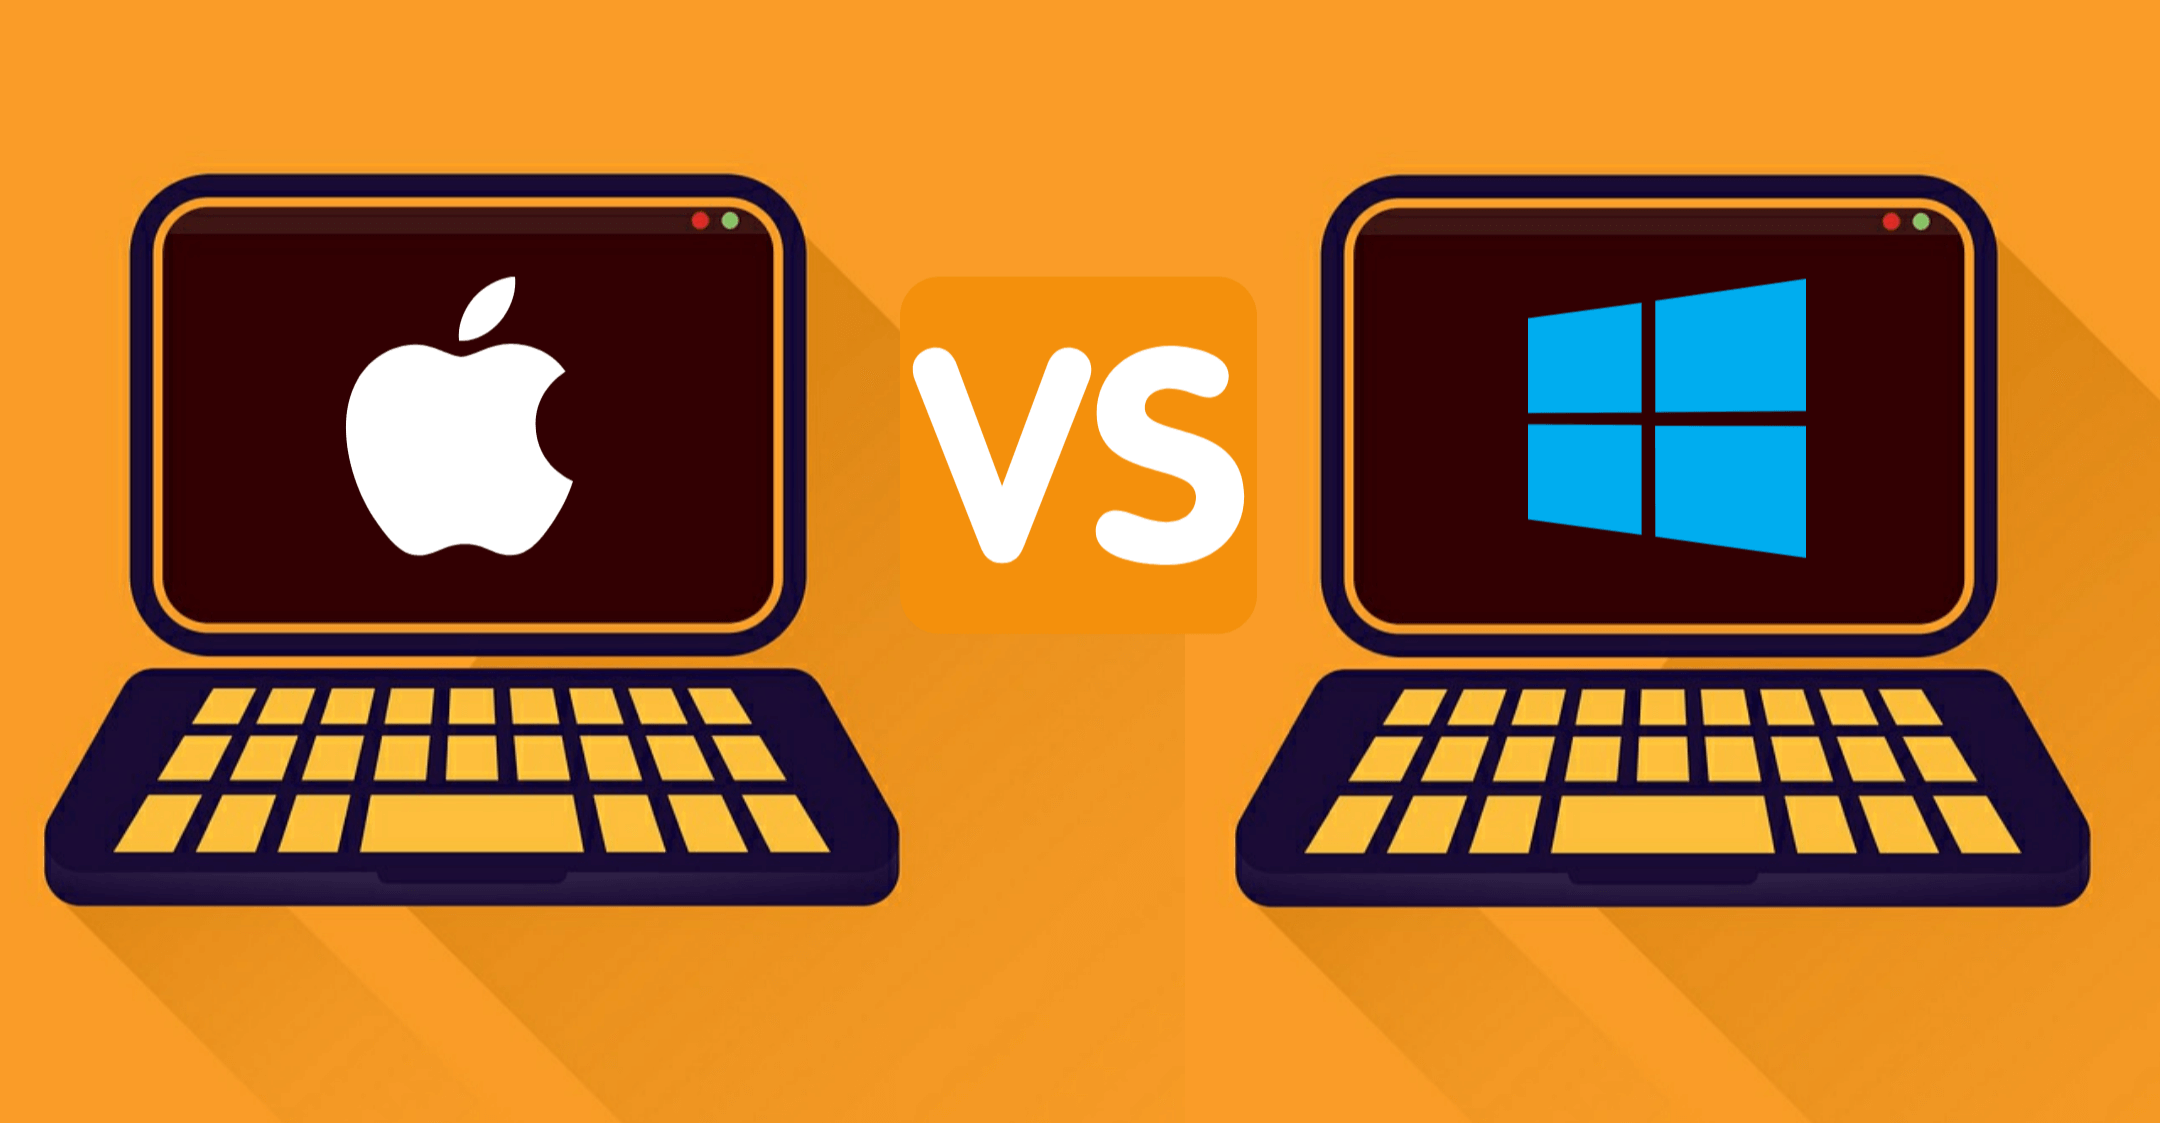
\includegraphics[scale=0.08]{mac_pc.png}
            }
            \only<7-8>{
              \includegraphics[scale=0.2]{étudiants.jpg}
            }
            \only<9-10>{
              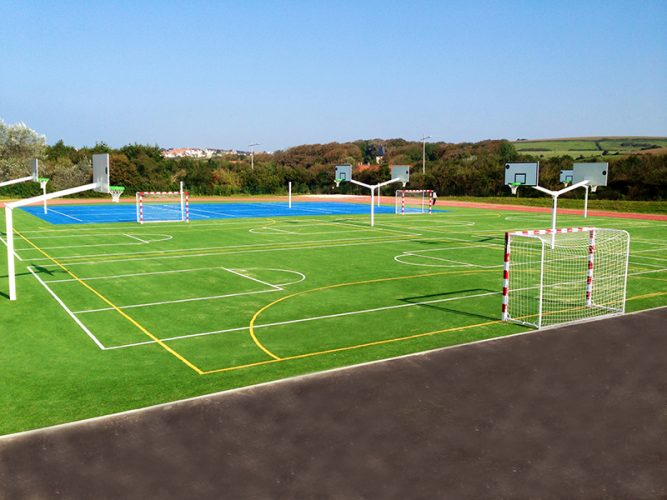
\includegraphics[scale=0.23]{terrains.jpg}
            }
            \only<11-12>{
              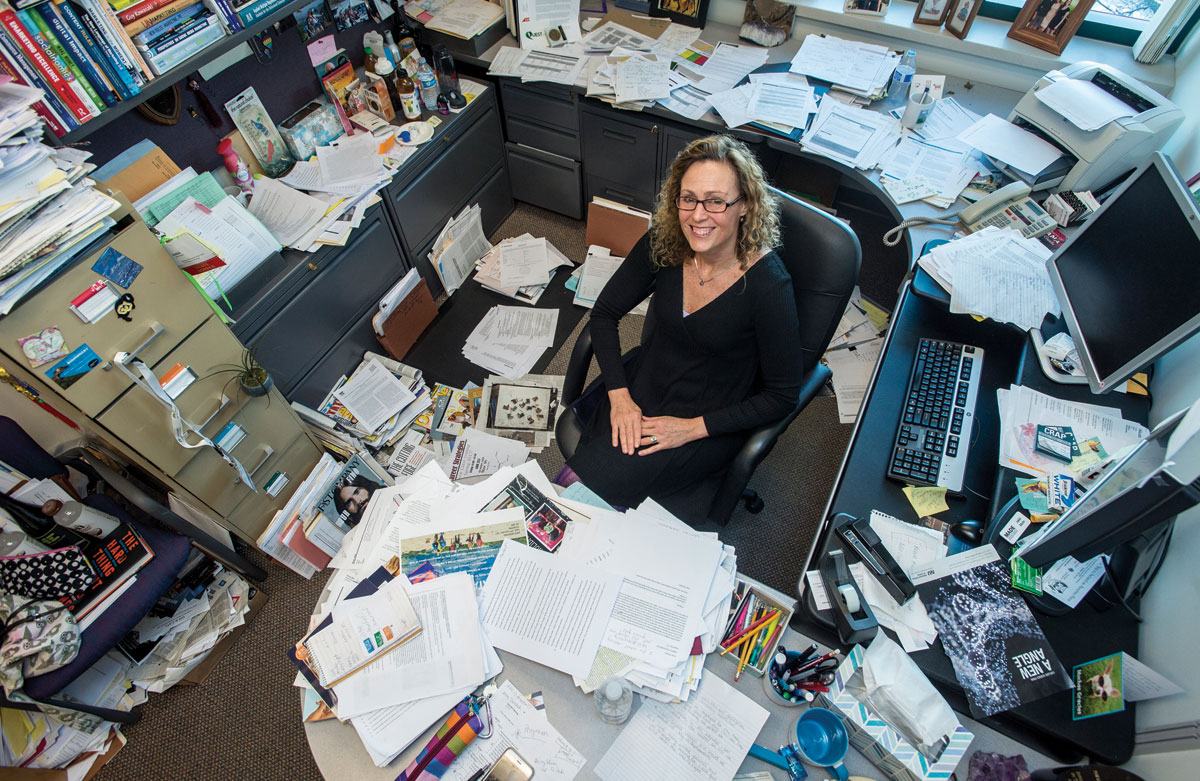
\includegraphics[scale=0.14]{bureau.jpg}
            }
            \only<13-14>{
              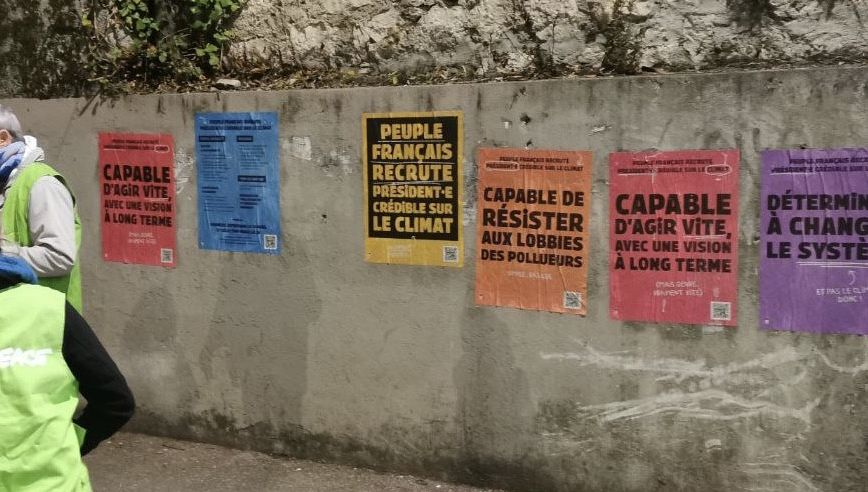
\includegraphics[scale=0.18]{affiches.jpg}
            }
            \only<15-16>{
              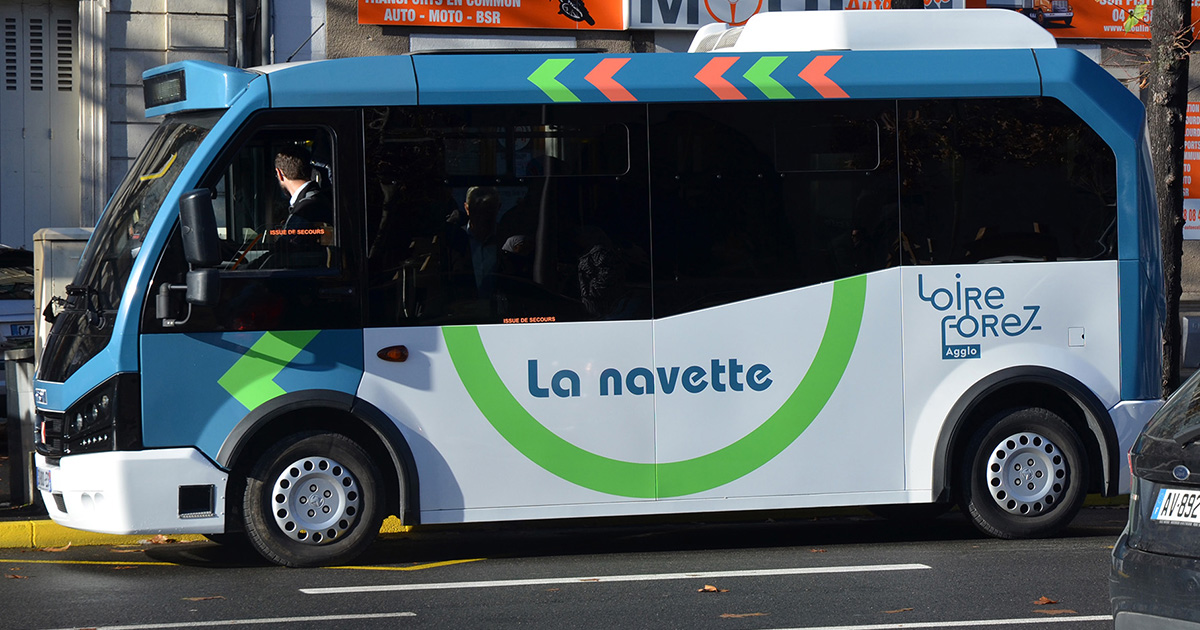
\includegraphics[scale=0.55]{navette.jpg}
            }
          \end{center}
        \end{minipage}
    \end{columns}
  \end{frame}

  \begin{frame}{Le travail à faire}
    En groupes de 3 à 5, comparez ce que vous faites dans vos cours cette semaine. \\
    \tinygloss{In groups of 3 to 5, compare what you're doing in your classes this week.}
    \begin{description}
      \item[] \textbf{Modèle:}
      \item[E1:] Moi, je prépare un exposé pour mon cours de sociologie, et j'ai deux examens vendredi.
      \item[E2:] Je n'ai pas d'examens, moi, mais je prépare un essai pour mon cours d'histoire et un gros projet pour mon cours de gestion.
      \item[E3:] Moi, je n'ai pas beaucoup de travail. Je fais des devoirs pour mon cours de psychologie. C'est tout.
    \end{description}
  \end{frame}

  \begin{frame}{Ma ville natale}
    Décris ta ville natale à un/e partenaire en décrivant le caractère des endroits suivants avec des adjectifs ainsi que leurs dispositions. \\
    \tinygloss{Describe your hometown to a partner by describing the character of the following places with adjectives as well as their locations.}
    \vspace{0.25cm}
    \begin{columns}[t]
      \column{0.4\textwidth}
        \begin{description}
          \item[] \textbf{Modèle:}
          \item[] \emph{des parcs}
          \item[E1:] Dans ma ville natale, il y a des jolis parcs dans le centre-ville.
        \end{description}
      \column{0.28\textwidth}
        \begin{enumerate}
          \item une mairie
          \item des parcs
          \item des hôtels
          \item des piscines municipales
        \end{enumerate}
      \column{0.32\textwidth}
        \begin{enumerate}
          \setcounter{enumi}{4}
          \item des universités
          \item des cinémas
          \item des maisons
          \item des appartements
        \end{enumerate}
    \end{columns}
  \end{frame}

  \begin{frame}{}
    \begin{center}
      \Large Questions?
    \end{center}
  \end{frame}
\end{document}
